\section{HIM Reproduction and Controlled Extensions}
\label{sec:him-experiments}
\subsection{Questions and contribution boundary}
The HIM component addresses three questions. Can the saved author-code pipeline be executed and independently re-evaluated? Does the ASW selector improve on the same representation without adaptive discounting? Can an explicit structural or cumulative-coverage rule improve the selected set? These are different questions: a successful reload is a reproducibility check, a same-checkpoint selector contrast is an ablation, and a new selector is a method extension. None alone establishes that a new representation model has been learned.

The original paper contributes hyperbolic influence representations, relation-specific fitting of social and activation edges, proactive activation regularization, the LDO proxy, and ASW \cite{him}. Our course work retains that architecture. The additions are execution and provenance fixes, independent evaluations, nine new training runs on original networks, a Ciao topology extension, and two explicit changes to the selection stage. Neighborhood discounting, coverage functions, and greedy/lazy evaluation have established foundations \cite{kempe,celf}; we do not claim those general ideas as literature-first inventions.

\subsection{Engineering work and reproducibility checks}
The first stage adapted the public implementation to the local Apple Silicon CPU environment and exposed dataset, exact seed budget, and random seed through the command line. Best checkpoints and their corresponding seed IDs are now saved together. A reload check reconstructs the seed set from the checkpoint and verifies it against the stored IDs before evaluating spread.

Several details matter for interpreting a successful run. Training-cache keys now include the graph hash, probability-bank identifier, sample ratio, seed budget, number of propagation instances, and training seed; the instance count is checked on loading. This prevents a short smoke-test cache from being silently reused as a 30-instance experiment. The diffusion base class resets NumPy's generator only when an explicit seed is supplied, allowing the caller to control independent evaluation streams. Node IDs are converted to Python integers when saved as JSON, since some original graphs expose NumPy integer neighbor IDs. The Power Grid WIC configuration also lacks the sample-ratio field required by the runner; the study explicitly sets it to 0.2. These are recorded implementation/configuration adaptations, not changes to the learned objective.

The historical Cora-ML check described earlier establishes checkpoint-to-seed-to-evaluation consistency. It uses one saved final-epoch model and must not be combined with a maximum online-validation score as though both were the same endpoint. The later studies below use independently trained models or frozen checkpoints and their own named evaluation streams.

\subsection{Expanded author-code reproduction}
Nine new models were trained: seeds 142, 143, and 144 on each of Cora-ML, Power Grid, and Facebook. Each uses 30 synthetic training cascades, at most 200 epochs, 100 online-validation simulations per epoch, and patience 10 under the existing runner's stopping rule. The best checkpoint selected by online validation is then frozen. The 10\% budget is implemented as $k=\lfloor0.1|V|\rfloor$, giving 281, 494, and 590 seeds respectively.

Three earlier Ciao models, trained with seeds 42, 43, and 44, use the same 30-instance regime and an exact budget of 366 users, approximately 5\%. The graph has 7,317 nodes and 85,205 undirected trust edges. Its propagation remains synthetic under the fixed degree-derived WIC rule. There are no observed information cascades or causal opinion-adoption labels in this dataset.

Table~\ref{tab:him-scope} separates the network and budget settings. Reproducing the author code is not an exact replication of every manuscript table. The paper describes WIC edge probabilities in $[0,0.2]$, whereas the supplied banks used here are approximately $[0.1,0.2]$ on Cora-ML and Power Grid and $[0,0.1]$ on Facebook. Ciao uses a different, topology-derived bank. The study does not cover GitHub/YouTube, the complete IC/LT/WIC/WLT matrix, all budgets, all paper baselines, or representation-learning ablations. MD removes ASW's selection adjustment; it does not remove hyperbolic geometry or activation regularization.

\begin{table}[t]
\centering\footnotesize
\caption{HIM settings. Each row has three independently trained models. Ciao checkpoints predate the nine new paper-network runs.}
\label{tab:him-scope}
\setlength{\tabcolsep}{3.5pt}
\begin{tabular}{@{}lrrr@{}}
\toprule
Network & Nodes & Edges & $k$ \\
\midrule
Cora-ML & 2,810 & 7,981 & 281 \\
Power Grid & 4,941 & 6,594 & 494 \\
Facebook & 5,908 & 41,729 & 590 \\
Ciao & 7,317 & 85,205 & 366 \\
\bottomrule
\end{tabular}
\end{table}

\subsection{Evaluation units and uncertainty}
Within a selector comparison, the model, graph, budget, probability bank, and simulator are fixed. For replicate $i$, Python and NumPy are reset to the same method-independent seed $b+i$. This gives paired initial random streams; it does not ensure that different seed sets consume a common random draw for each edge. The simulation follows the original implementation, including its maximum of 100 propagation steps.

The expanded three-network study uses $R=500$ replicates with seed base $b=100042$. The earlier Ciao study uses $R=1,000$ and $b=1042$. A paired contrast is first computed within each checkpoint. If $d_j$ is the mean activated-user difference for training model $j$, the across-model interval is
\begin{equation}
\bar d\ \pm\ t_{0.975,2}\frac{s_d}{\sqrt{3}},
\qquad j\in\{1,2,3\}.
\end{equation}
The independent unit in this interval is the trained model, not a propagation replicate. More simulations reduce conditional Monte Carlo noise but do not create additional trained models. Three models remain a small sample. No multiplicity correction was prespecified, so intervals throughout this section are unadjusted exploratory summaries.

ASW and MD are reselected from the same frozen representation. Degree selects the largest-degree nodes with deterministic ID tie-breaking; Random samples a budget-sized set using the recorded seed. Degree is one fixed set per network, and Random's variation is seed-set sampling rather than model training. Identical sets under identical evaluation conditions may reuse outcomes, with the source recorded; this is not extra independent evidence.

\subsection{First extension: neighborhood-overlap ASW-J}
The initial extension keeps ASW's window, graph-neighbor candidate restriction, and total discount scale. For current seed $c$ and eligible candidate $v$, it computes open-neighborhood Jaccard overlap,
\begin{equation}
J(c,v)=\frac{|N(c)\cap N(v)|}{|N(c)\cup N(v)|}.
\end{equation}
When at least one overlap is nonzero, the new attention is
\begin{equation}
w_{cv}=(1-\alpha)w^{\mathrm{geom}}_{cv}
+\alpha\frac{J(c,v)}{\sum_{z}J(c,z)},\quad \alpha=0.5.
\end{equation}
The original geometric attention is retained if no structural evidence is available. The mixing weight was fixed before evaluating outcomes. Other $\alpha$ values were used only to diagnose seed-set changes, not to select the best-performing parameter.

Table~\ref{tab:him-first-controls} records the expanded controls. In Facebook, Random's observed mean is slightly above the three HIM selectors, illustrating that topology and propagation assumptions matter. The ASW-J--ASW across-model intervals in Table~\ref{tab:aswj} all include zero. The changed-seed counts are only $[2,2,1]$ on Cora-ML, $[6,10,8]$ on Power Grid, $[1,1,3]$ on Facebook, and $[1,2,1]$ on Ciao. Retaining the original window and penalty scale may limit the intervention, but that mechanism has not itself been isolated by an ablation.

\begin{table}[t]
\centering\scriptsize
\setlength{\tabcolsep}{3pt}
\caption{First extension study: mean coverage (\%) across three paper-network models, 500 simulations/set, stream 100042.}
\label{tab:him-first-controls}
\begin{tabular}{@{}lrrrrr@{}}
\toprule
Network & ASW & MD & ASW-J & Degree & Random \\
\midrule
Cora-ML & 38.1440 & 37.6479 & 38.1832 & 34.3678 & 37.8651 \\
Power Grid & 18.7217 & 18.2440 & 18.7218 & 18.2193 & 15.2432 \\
Facebook & 31.8099 & 31.8031 & 31.8312 & 26.5291 & 31.9168 \\
\bottomrule
\end{tabular}
\end{table}

\begin{table}[t]
\centering\footnotesize
\setlength{\tabcolsep}{4pt}
\caption{ASW-J minus ASW: activated users, across-model 95\% $t$ intervals. Ciao uses its earlier stream 1042.}
\label{tab:aswj}
\begin{tabular}{@{}lrr@{}}
\toprule
Network & Mean difference & 95\% interval \\
\midrule
Cora-ML & $+1.102$ & $[-0.754, 2.958]$ \\
Power Grid & $+0.008$ & $[-1.707, 1.723]$ \\
Facebook & $+1.263$ & $[-2.237, 4.762]$ \\
Ciao & $-0.319$ & $[-2.074, 1.436]$ \\
\bottomrule
\end{tabular}
\end{table}

\subsection{Second extension: cumulative coverage HIM-C}
The second extension replaces local pairwise discounting with an explicit estimate of coverage by the complete selected set. Candidate selection is global rather than confined to the original window. We retain the trained embedding and define $h(v)\in[0,1]$ as the reversed percentile rank of LDO: lower LDO gives higher $h$, and equal scores receive average ranks. For adjacent distinct nodes, define
\begin{equation}
q_{vu}=p_0\big[(1-\lambda)+\lambda h(v)\big],
\quad p_0=0.1,\ \lambda=0.5.
\end{equation}
Self-coverage is $q_{vv}=1$, and $q_{vu}=0$ for non-neighbors. These are surrogate probabilities, not estimates read from the evaluator's true probability file. Both constants are fixed across all four networks before the study. In particular, the selector receives neither test outcomes nor the true Ciao edge probabilities.

For a selected set $S$, let
\begin{align}
r_S(u)&=\prod_{v\in S}(1-q_{vu}),\\
F(S)&=\sum_{u\in V}[1-r_S(u)].
\end{align}
Here $r_S(u)$ is the surrogate probability that $u$ remains uncovered. Adding candidate $v$ gives the exact marginal of this one-hop surrogate,
\begin{equation}
\Delta_F(v\mid S)=r_S(v)+q_v\sum_{u\in N(v),u\ne v}r_S(u),
\end{equation}
where $q_v=p_0[(1-\lambda)+\lambda h(v)]$. HIM-C repeatedly takes the largest marginal among all unselected nodes, then updates the residual vector. We use lazy re-evaluation of decreasing marginal upper bounds, an established acceleration principle \cite{celf}. Small-graph exhaustive marginal scans verify the selected sequence. Facebook self-loops are ignored only inside this coverage surrogate because self-coverage is already one; the original graph, embedding, and evaluation simulator are unchanged.

The surrogate models independent direct coverage, whereas the evaluator permits multi-hop cascades. Even if the surrogate has diminishing returns, that does not transfer a greedy performance guarantee to the actual diffusion objective. The graph-based kernel, the fixed probability scale, and the rank mapping are explicit modeling assumptions.

\subsection{Coverage-only control and attribution}
The CO control uses the identical global greedy procedure and cumulative-coverage objective with $\lambda=0$, so every graph edge uses $p_0=0.1$. It removes the HIM prior as a component while retaining the coverage mechanism. It is not an equal-average-probability control: removing the modulation changes both heterogeneity and average surrogate intensity. Consequently, this ablation can test whether the current HIM-prior configuration adds practical benefit, but cannot establish that all learned influence information is useless. The experiment also changes candidate scope and the selection objective together; it does not separately identify their contributions.

\subsection{Independent selector validation results}
The HIM-C study freezes all 12 existing checkpoints and uses a new seed base, $b=200042$, with 500 simulations per set. ASW is reevaluated on that same stream. The ASW scores here therefore differ slightly from earlier tables due to evaluation randomness and replicate count; differences are always computed within the same protocol. No encoder is retrained and no parameter is chosen using these results.

Table~\ref{tab:coverage-results} gives the coverage means. Relative to ASW, the unadjusted across-model intervals for HIM-C are positive on Power Grid, Facebook, and Ciao, but include zero on Cora-ML. These are conditional improvements, not a universal advantage. Figure~\ref{fig:coverage-contrasts} shows why reporting the CO ablation changes the interpretation: CO is higher than HIM-C on Power Grid and Facebook, and neither of the other networks provides a stable positive HIM-prior contrast. The supported finding is that the tested global cumulative-coverage strategy improves ASW in some settings; an additional benefit from the particular HIM prior remains unsupported.

\begin{table}[t]
\centering\footnotesize
\setlength{\tabcolsep}{5pt}
\caption{New-stream validation: mean coverage (\%), 500 simulations/set, stream 200042. Each network has three frozen HIM models.}
\label{tab:coverage-results}
\begin{tabular}{@{}lrrr@{}}
\toprule
Network & ASW & HIM-C & CO \\
\midrule
Cora-ML & 38.1071 & 37.9670 & 38.0662 \\
Power Grid & 18.7235 & 20.5250 & 20.6025 \\
Facebook & 31.8542 & 32.2035 & 32.3416 \\
Ciao & 10.0150 & 10.5933 & 10.5762 \\
\bottomrule
\end{tabular}
\end{table}

\begin{table*}[t]
\centering\small
\caption{New-stream paired contrasts in activated users. Intervals are across three trained models ($df=2$), not across 500 simulations. All intervals are unadjusted.}
\label{tab:coverage-contrasts}
\setlength{\tabcolsep}{12pt}
\begin{tabular}{@{}lrrrr@{}}
\toprule
Network & HIM-C $-$ ASW & 95\% interval & HIM-C $-$ CO & 95\% interval \\
\midrule
Cora-ML & $-3.937$ & $[-23.664, 15.790]$ & $-2.788$ & $[-7.027, 1.451]$ \\
Power Grid & $+89.013$ & $[80.360, 97.665]$ & $-3.830$ & $[-5.345, -2.315]$ \\
Facebook & $+20.638$ & $[3.182, 38.094]$ & $-8.161$ & $[-9.484, -6.839]$ \\
Ciao & $+42.315$ & $[35.478, 49.152]$ & $+1.250$ & $[-0.462, 2.962]$ \\
\bottomrule
\end{tabular}
\end{table*}

\begin{figure*}[t]
\centering
\begin{minipage}{0.49\textwidth}\centering
\begin{tikzpicture}\begin{axis}[
width=0.90\linewidth,height=5.5cm,title={HIM-C minus ASW},xmin=-40,xmax=120,xtick={-40,0,40,80,120},ymin=0.5,ymax=4.5,ytick={1,2,3,4},yticklabels={Ciao,Facebook,Power Grid,Cora-ML},xlabel={Additional activated users},axis y line*=left,y axis line style={draw=none},ytick style={draw=none},axis x line*=bottom,xmajorgrids=true,grid style={gray!15},tick align=outside,tick label style={font=\scriptsize},label style={font=\scriptsize},title style={font=\small},scale only axis=false]
\addplot[gray!60,dashed,no marks] coordinates {(0,0.5) (0,4.5)};
\addplot+[only marks,mark=*,mark size=2pt,blue!65!black,mark options={fill=blue!65!black,draw=blue!65!black},error bars/.cd,x dir=both,x explicit,error bar style={blue!65!black},error mark options={line width=0.7pt}] coordinates {
(-3.936666667,4) +- (19.726990586,0)
(89.012666667,3) +- (8.652594107,0)
(20.638000000,2) +- (17.455544134,0)
(42.315333333,1) +- (6.837076900,0)
};\end{axis}\end{tikzpicture}\end{minipage}
\begin{minipage}{0.49\textwidth}\centering
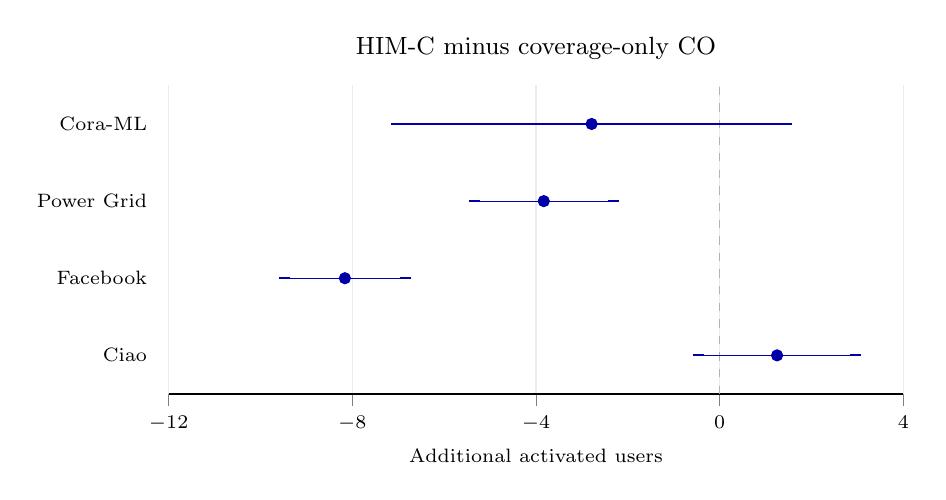
\begin{tikzpicture}\begin{axis}[
width=0.90\linewidth,height=5.5cm,title={HIM-C minus coverage-only CO},xmin=-12,xmax=4,xtick={-12,-8,-4,0,4},ymin=0.5,ymax=4.5,ytick={1,2,3,4},yticklabels={Ciao,Facebook,Power Grid,Cora-ML},xlabel={Additional activated users},axis y line*=left,y axis line style={draw=none},ytick style={draw=none},axis x line*=bottom,xmajorgrids=true,grid style={gray!15},tick align=outside,tick label style={font=\scriptsize},label style={font=\scriptsize},title style={font=\small},scale only axis=false]
\addplot[gray!60,dashed,no marks] coordinates {(0,0.5) (0,4.5)};
\addplot+[only marks,mark=*,mark size=2pt,blue!65!black,mark options={fill=blue!65!black,draw=blue!65!black},error bars/.cd,x dir=both,x explicit,error bar style={blue!65!black},error mark options={line width=0.7pt}] coordinates {
(-2.788000000,4) +- (4.239089114,0)
(-3.830000000,3) +- (1.515193683,0)
(-8.161333333,2) +- (1.322171261,0)
(1.250000000,1) +- (1.711655609,0)
};\end{axis}\end{tikzpicture}\end{minipage}

\caption{HIM-C contrasts under the same new evaluation stream. Points show mean activated-user differences and lines show unadjusted 95\% $t$ intervals across three frozen training models. Budgets are 10\% on the first three networks and approximately 5\% on Ciao. Panels use different horizontal scales; networks are not pooled. The CO comparison does not support a stable additional gain from the present HIM-prior configuration.}
\label{fig:coverage-contrasts}
\end{figure*}

\subsection{Checks, retained evidence, and practical interpretation}
The coverage audit verifies graph, probability-bank, source-result, checkpoint, selector, and simulator hashes. It reloads all 12 checkpoints, recomputes HIM-C and CO sets, and checks cardinality, bounds, outcome means, within-model paired intervals, and across-model intervals. The archived new-stream study contains 14,000 non-reused propagation simulations; repeated deterministic CO sets are evaluated once per network under that stream and reused with recorded provenance. Earlier failed or interrupted attempts are not counted as extra evidence.

Separately, the geometric implementation control forces structural blending off and recovers exactly the original ASW set on all 12 checkpoints used in the earlier ASW-J study. This checks refactoring effects on those models, not every possible input. Twenty scoped behavior/statistics tests cover the two selector extensions, tie handling, invalid inputs, budgets, isolates, and the distinction between model-level and replicate-level uncertainty.

Our main practical lesson is methodological. A representation can provide a plausible individual ranking while leaving set-level coverage poorly controlled. Modifying the selector can improve that behavior without improving the representation itself. Keeping the unsuccessful ASW-J result and the less favorable CO ablation makes the contribution inspectable: it records what was changed, what improved under fixed conditions, and which explanation the evidence does not support.
